\documentclass{beamer}

\usepackage[utf8]{inputenc}
\usepackage{fancybox,fancyvrb}
\usepackage{environ}
\usepackage{tikz}

\beamertemplatenavigationsymbolsempty
\setbeamertemplate{footline}[frame number]
\usetheme{Pittsburgh}

\newcommand\enumnum[1]{{\renewcommand{\insertenumlabel}{#1}%
      \usebeamertemplate{enumerate item} \,}}

\newcommand{\grad}{\nabla}
\newcommand{\ih}{\boldsymbol{\hat{\textbf{\i}}}}
\newcommand{\jh}{\boldsymbol{\hat{\textbf{\j}}}}
\newcommand{\vF}{\boldsymbol{\vec{\textbf{F}}}}


\title{3.1 Linear Models}

\subtitle{a lesson for MATH F302 Differential Equations}

\author{Ed Bueler, Dept.~of Mathematics and Statistics, UAF}

\date{\tiny \today}


\begin{document}
\setbeamertemplate{itemize item}{$\bullet$}
\setbeamertemplate{itemize subitem}{$\circ$}

\begin{frame}
\titlepage

\centerline{\tiny for textbook: \, D. Zill, \emph{A First Course in Differential Equations with Modeling Applications}, 11th ed.}
%\color{green!40!blue}
\end{frame}


\begin{frame}{linear models}

\begin{itemize}
\item not new material?
    \begin{itemize}
    \item we got a good start back in \S1.3
    \end{itemize}
\item this section requires ability to solve these types of DEs:
    \begin{enumerate}
    \item the easiest DE: $y'=ky$
    \item separable linear equations from \S2.2: $y'=g(x)y$ or $y'=ay+b$
    \item general linear equations from \S2.3: $y'+P(x)y=f(x)$                 
    \end{enumerate}
\item \dots which should be easy at this point
\item the method in \S2.3 handles all first-order \emph{linear} equations, but the other methods are usually quicker for forms \enumnum{1} or \enumnum{2}
\item these slides simply contain 5 exercises from \S3.1 in this order:

\hspace{20mm} \# 4, 42, 17, 36, 37
\end{itemize}
\end{frame}


\begin{frame}{exercise 4}

\small
\begin{quotation}
\noindent \textbf{4.} The population of bacteria in a culture grows at a rate proportional to the number of bacteria present at time $t$.  After 3 hours it is observed that 400 bacteria are present.  After 10 hours 2000 bacteria are present.  What was the initial number of bacteria?
\end{quotation}

\vspace{50mm}
\end{frame}


\begin{frame}{exercise 42}

\small
\begin{quotation}
\noindent \textbf{42.  Fluctuating Population} \, The differential equation $dP/dt = (k \cos t) p$, where $k$ is a positive constant, is a mathematical model for a population $P(t)$ that undergoes yearly seasonal fluctuations.  Solve the equation subject to $P(0)=P_0$.  Use a graphing utility to graph the solution for different choices of $P_0$ [and $k$]. 
\end{quotation}

\vspace{45mm}
\end{frame}


\begin{frame}{exercise 42, cont.}

\vspace{30mm}

\hfill 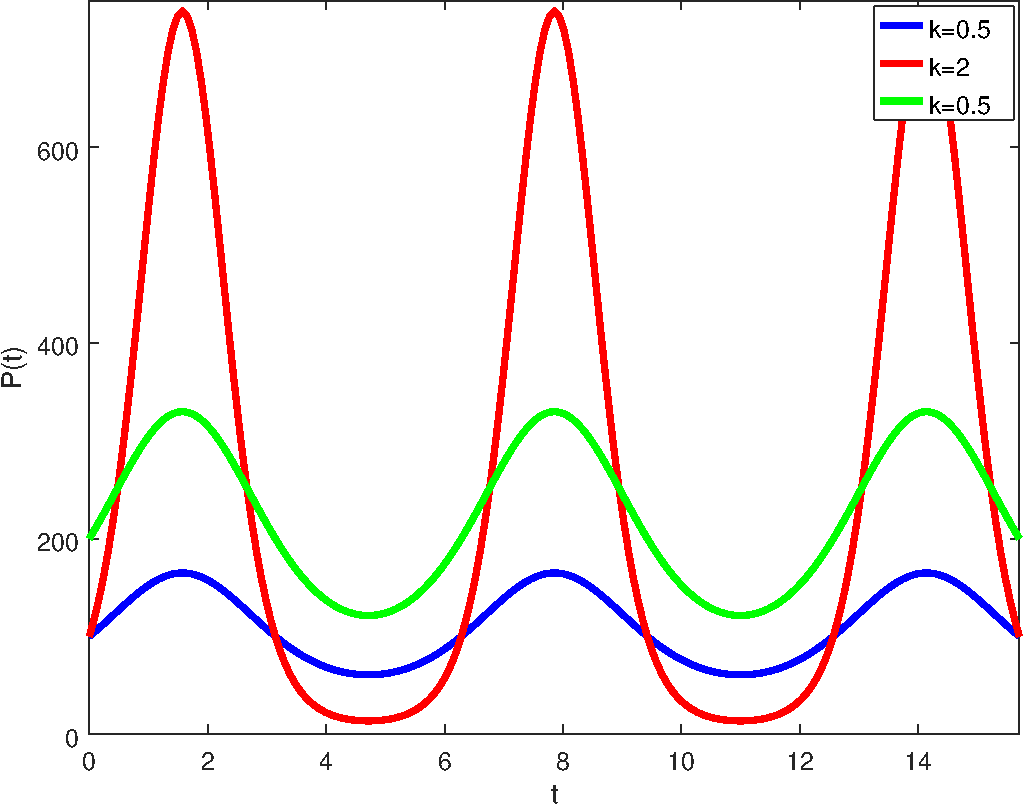
\includegraphics[width=0.5\textwidth]{figs/exercise-42-3-1}
\end{frame}


\begin{frame}{exercise 17}

\small
\begin{quotation}
\noindent \textbf{17.} A thermometer reading $70^\circ$F is placed in an oven preheated to a constant temperature.  Through a glass window in the oven door, an observer records that the thermometer reads $110^\circ$F after $\frac{1}{2}$ minute and $145^\circ$F after 1 minute.  How hot is the oven?
\end{quotation}

\vspace{50mm}
\end{frame}


\begin{frame}{X}

\begin{itemize}
\item X
\end{itemize}
\end{frame}


\begin{frame}{exercise 36}

\begin{minipage}[t]{0.75\textwidth}
\small
\begin{quotation}
\noindent \textbf{36. How High?---No Air Resistance} \, Suppose a small cannonball weighing 16 pounds is shot vertically upward, as shown in the Figure, with an initial velocity $v_0 = 300 \text{ft}/\text{s}$.  The answer to the question ``How high does the cannonball go?'' depends on whether we take air resistance into account.

\noindent \textbf{(a)} \, Suppose air resistance is ignored.  If the positive direction is upward then a model for the height $s(t)$ of the cannonball is given by $m d^2s/dt^2 = - mg$ or equivalently $d^2s/dt^2 = - g$.  Since $ds/dt = v(t)$ the last differential equation is the same as $dv/dt = -g$.  We take $g=32 \text{ft}/\text{s}^2$.  Find the velocity $v(t)$ of the cannonball at time $t$.
\end{quotation}
\end{minipage}
\begin{minipage}[t]{0.25\textwidth}
\vspace{0mm}
FIXME
\end{minipage}
\end{frame}


\begin{frame}{exercise 36, cont.}

\small
\begin{quotation}
\noindent \textbf{(b)} \, Use the result in part \textbf{(a)} to determine the height $s(t)$ of the cannonball, measured from ground level.  Find the maximum height attained by the cannonball.
\end{quotation}

\vspace{50mm}
\end{frame}


\begin{frame}{X}


\begin{itemize}
\item X
\end{itemize}
\end{frame}


\begin{frame}{exercise 37}

\begin{quotation}
\noindent \textbf{37.  How High?---Linear Air Resistance}  FIXME
\end{quotation}

\vspace{50mm}
\end{frame}


\begin{frame}{X}

\begin{itemize}
\item X
\end{itemize}
\end{frame}


\begin{frame}{expectations}

\begin{itemize}
\item to learn this material, just watching this video is \emph{not} enough!

\item also:
     \begin{itemize}
     \item \emph{explore} ``found online'' videos at

     \centerline{\href{https://bueler.github.io/math302/week5.html}{\tt \color{cyan} bueler.github.io/math302/week5.html}}
     \item \emph{read} section 3.1 in the textbook
         \begin{itemize}
         \item for quizzes and exams you must be able to handle the \underline{examples} like 1-6 in this section
         \item \dots and \underline{exercises} like those in WebAssign
         \item one topic you will not be responsible for: ``series circuits'' and other electical examples
         \end{itemize}
     \item \emph{do} the WebAssign exercises for section 3.1
     \item \emph{start} Mini-Project 2, which uses a model like in section 3.1
     \end{itemize}
\end{itemize}
\end{frame}

\end{document}

